\documentclass{article}
\usepackage[utf8]{inputenc}
\usepackage[spanish]{babel}
\usepackage{listings}
\usepackage{graphicx}
\usepackage{geometry}
\graphicspath{ {images/} }
\usepackage{cite}

\geometry{
textheight=23cm
}
\begin{document}

\begin{titlepage}
    \begin{center}
        \vspace*{0cm}
            
        \Huge
        \textbf{Parcial 1}
            
        \vspace{0.5cm}
        \LARGE
        Informa2 S.A.S.
            
        \vspace{5cm}
            
        \textbf{David Agudelo Ochoa}
        
        \vspace{0.5cm}
        
        \textbf{Juan Pablo Cruz Gómez}
        
        \vspace{0.5cm}
        
        \textbf{Erika Dayana León Quiroga}
            
        \vfill
            
        \vspace{0.8cm}
            
        \Large
        Despartamento de Ingeniería Electrónica y Telecomunicaciones\\
        Universidad de Antioquia\\
        Medellín\\
        Marzo de 2021
            
    \end{center}
\end{titlepage}

\tableofcontents
\newpage
\section{Sección introductoria.}\label{intro}
Este informe se hace con la intención de mostrar la solución de un problema cotidiano mediante el uso de  estructuras de programación, tipos de datos, funciones, arreglos y apuntadores usados en el lenguaje C++, además de introducir los conocimientos adquiridos sobre el Arduino, y lograr trabajar con estas dos herramientas para mostrar la propuesta implementada en el software de simulación de circuitos Tinkercad.

\section{Análisis del problema.} \label{contenido}
En este problema, haciendo uso de tinkercad, se pide realizar la simulación de un circuito que controle un sistema compuesto por 64 LEDs (8 filas por 8 columnas) con ayuda de un arduino y la cantidad de circuitos integrados de registro de desplazamiento 74HC595 necesarios para su óptimo funcionamiento. El sistema compuesto por LEDs le mostrará al usuario el patrón de un caracter que él desee observar, el usuario podrá escribir palabras y el sistema se encargará de mostrar letra por letra, éstas separadas por un delay que el usuario escogerá a su gusto.
\subsection{Consideraciones iniciales}
Se debe tener en cuenta, según las restricciones, que se podrán usar máximo siete pines digitales del Arduino, se usarán dos circuitos integrados, cada uno de estos necesita tres pines digitales, uno de ellos controla las ocho filas y el otro las ocho columnas en el sistema compuesto por 64 LEDs. El pin sobrante, llamado Shift Register Clear, podrá ser utilizado como reset de la matriz de LEDs.


\subsection{Incluir código en el documento}
\section{Tareas para el desarrollo del problema} \label{imagenes}
\begin{enumerate}
  \item Comprender el funcionamiento del único circuito integrado que se puede utilizar para la solución de este problema, el 74HC595. (\ref{fig:Funcionamiento74HC595}),(\ref{fig:setup})
  
 \begin{figure}[h]
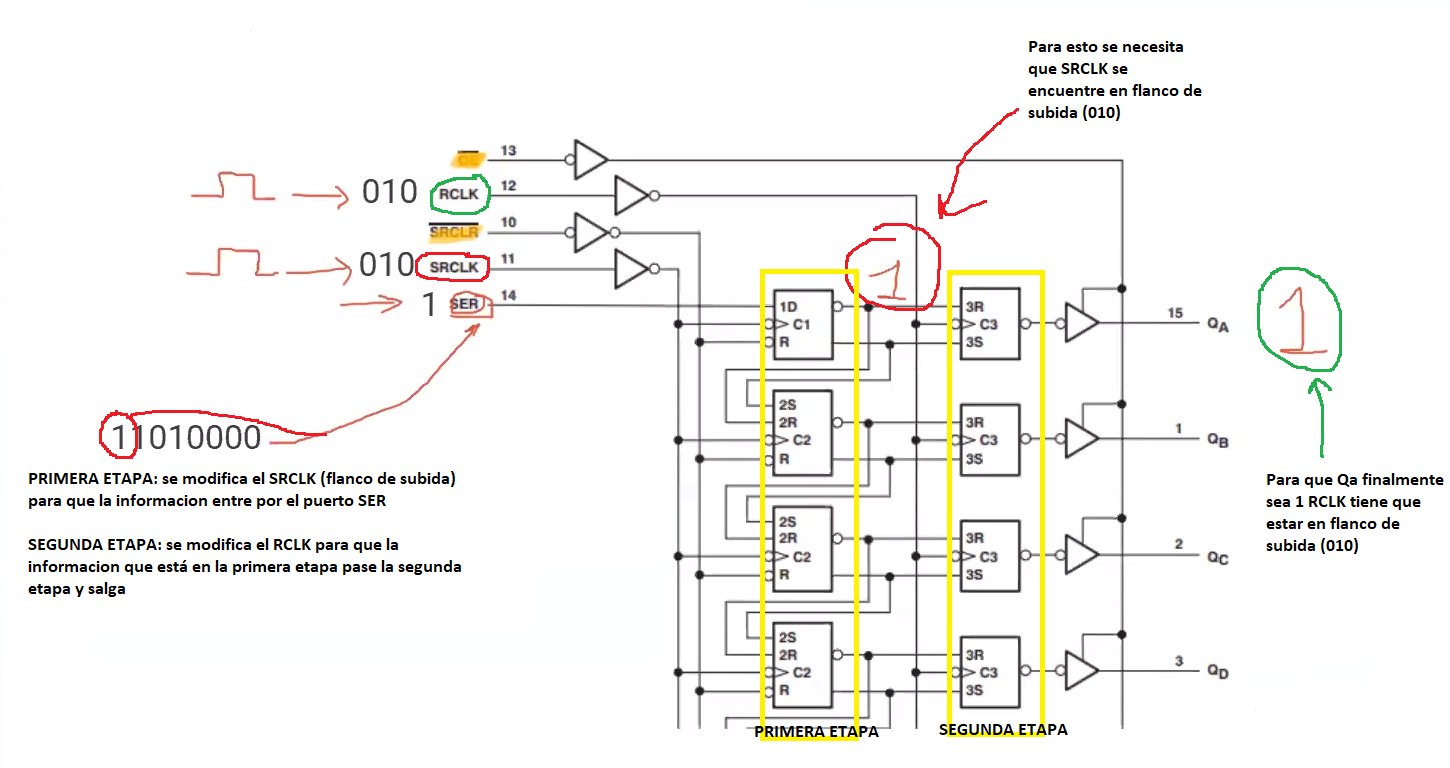
\includegraphics[scale=0.4]{FUNCIONAMIENTO74HC595.png}
\centering
\caption{Diagrama muestra el funcionamiento interno de un 74HC595.}
\label{fig:Funcionamiento74HC595}
\end{figure}
\newpage

\begin{figure}[h]
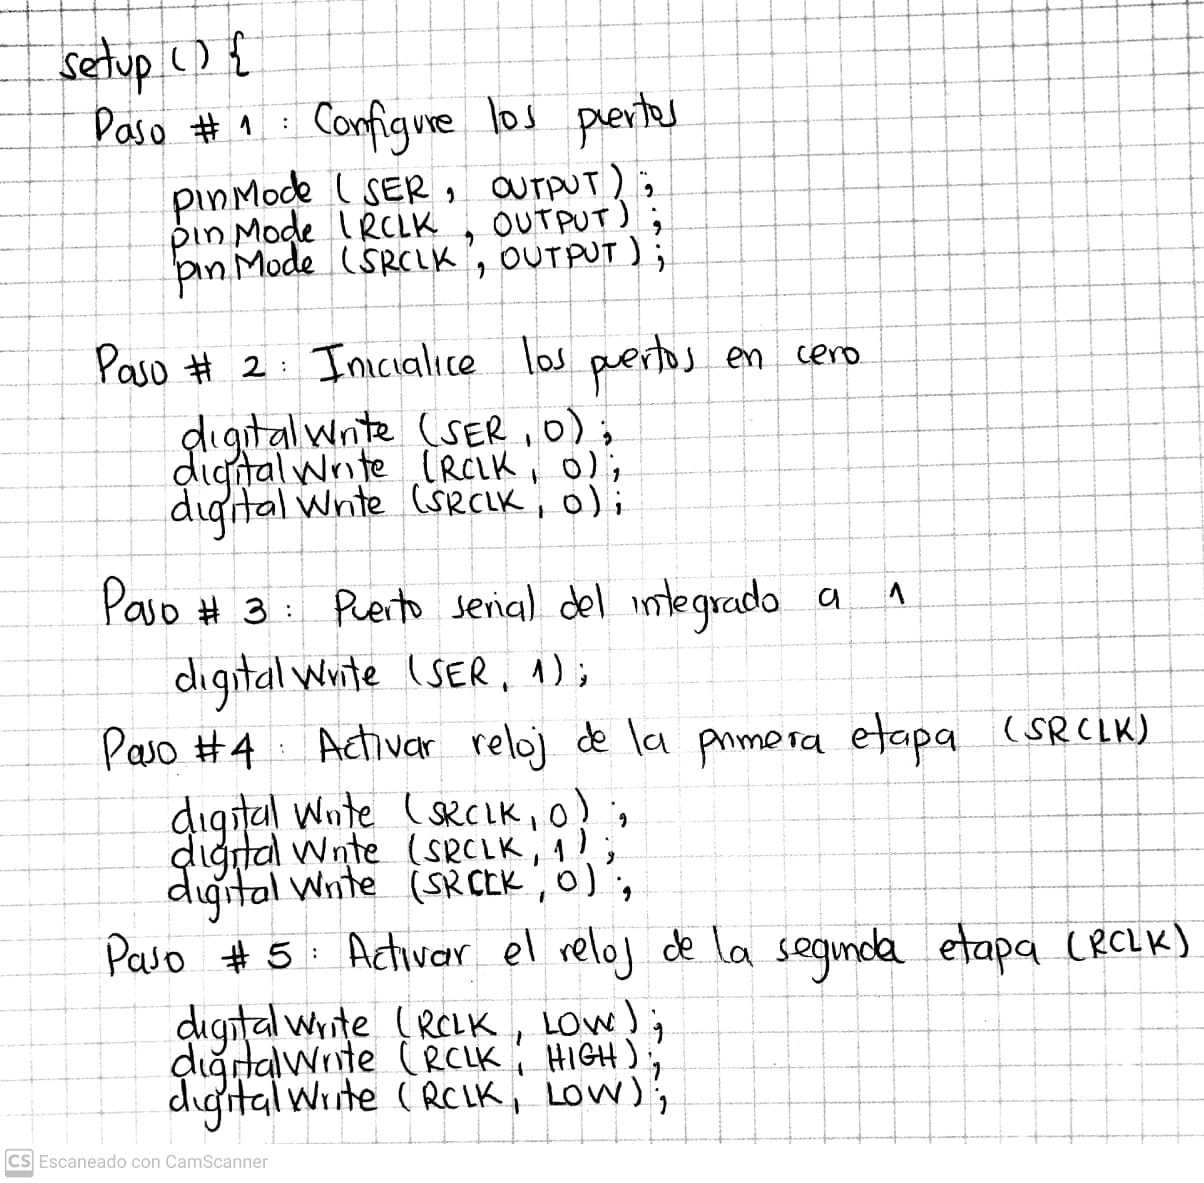
\includegraphics[width=10cm]{SETUP.jpeg}
\centering
\caption{Configuración del integrado 74HC595 en Tinkercad, teniendo en cuenta los pines utilizados del arduino.}
\label{fig:setup}
\end{figure}

  \item Realizar el montaje del circuito en la plataforma Tinkercad, recordando que se puede usar únicamente un arduino y un solo tipo de circuito integrado (74HC595).

  \begin{figure}[h]
  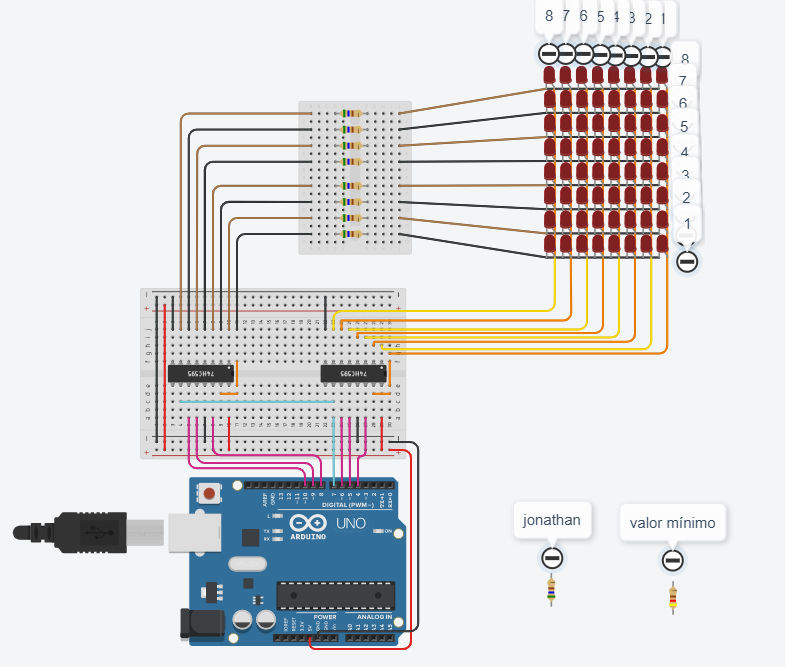
\includegraphics[width=6cm]{montaje1.png}
  \centering
  \caption{Primer montaje del circuito en Tinkercad}
  \label{fig:montaje1}
  \end{figure}
  \newpage
  \item Realizar una función que verifique el funcionamiento de la matriz de LEDs encendiendo a todos ellos por un tiempo determinado.
  \item Hacer una función que le pida al usuario la matriz de 8x8 conformada por unos y ceros que luego se verá reflejada en los LEDs.
  \item Crear una función llamada Publik que le permite al usuario observar la secuencia de patrones con un delay asignado por el mismo usuario.
  
  \begin{figure}[h]
  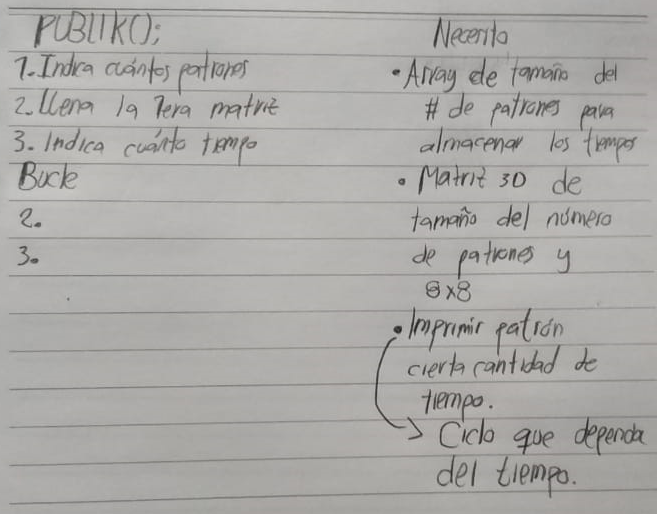
\includegraphics[scale=1]{publik.png}
  \centering
  \caption{Análisis para el desarrollo de la función publik()}
  \label{fig:publik}
  \end{figure}
  
  \item Hacer el manual de usuario en donde se tratará de explicar a detalle cómo funciona el sistema.
\end{enumerate}


\section{Algoritmo implementado} \label{imagenes}
(Hacer el mapa mental)
\section{Problemas durante el desarrollo del desafío}
\begin{itemize}
\item Al inicio de la implementación del código nos enfocamos en la creación de las funciones sin tener en cuenta la interacción que debía tener el usuario con el programa por medio de un menú, el usuario debía tener la capacidad de decidir ciertos aspectos relacionados con la visualización de los patrones en la matriz de LEDs, tales como el tiempo de visualización de cada patrón. Esto ocasionó la inevitable reestructuración de varias funciones para lograr la necesaria interacción del usuario.
\item Otro de los problemas presentados fue el querer implementar el concepto de la persistencia retiniana y la multiplexación tomando led por led, entonces se usaban las posiciones de una fila y se pedía encender el led de una de esas posiciones, el programa tomaba el uno y lo guardaba en la posición deseada y las demás posiciones eran rellenadas con ceros, al momento de querer enviar otro uno a otra posición de la misma fila ocurría que el primer uno enviado no se eliminaba sino que, teniendo en cuenta el funcionamiento de integrado 74HC595, se corría a una nueva posición en esa misma fila en donde probablemente no hiría un uno sino un cero.
\end{itemize}
\label{imagenes}
\section{Evolución del algoritmo} \label{imagenes}
sábado 17: inicialmente se implementó el montaje realizado por el profesor jonathan, posterior a ello se estudió cómo está conformada una matriz de leds, lo que llevó a estudiar terminos tales como la multiplexación y la persistencia. Conociendo esto, se procedió a montar la matriz de leds junto con los dos integrados y el arduino, haciendo uso inicialmente de 7 pines dígitales de este modo:

\begin{figure}[h]
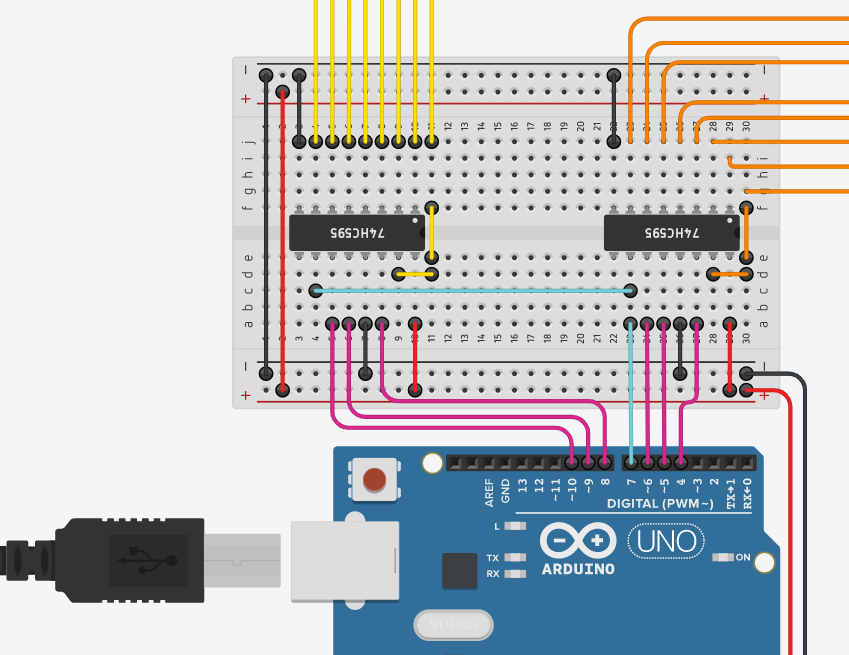
\includegraphics[scale=0.5]{pinesarduino.png}
\centering
\caption{Conexión al arduino de dos circuitos integrados 74HC595}
\label{fig:pinesarduinos}
\end{figure}

Domingo 18: se decidió que antes de empezar a programar, era importante entender cómo prender un led, por lo que se desarrollaría una función para encender un led, y aplicando el concepto de la persistencia del ojo humano, se conseguiría el cometido. Sin embargo, una vez se llegó a esta solución, se descubrió que presentaba discrepancias al querer encender varios leds en una misma fila. 
\newline
Lunes19: en horas de la mañana se desarrolla una función la cual permite encender filas de led, sin embargo, esta no tenía implementada una recepción por consola, y presentaba dificultades si el número ingresado desde el algoritmo empezaba con ceros.
 En horas de la tarde se construye primeramente una función para que el usuario ingrese por consola un numero de 8 digitos (compuesto únicamente de 1 y 0), y se almacene en un arreglo de tipo entero. Luego se usa la función obtenida para  llenar otro arreglo que contenga 8 arreglos en su interior, es decir, una matriz de 8x8, que además se le mostrará al usuario.
 Finalmente, se logra construir una función cuyo una de sus entradas será la matriz obtenida, permitiendonos así iluminar la matriz de leds de acuerdo a los 1 y 0 contenidos en nuestra matriz.
 Además se descubré que no hay necesidad de usar un pin individual para cada output register clock, pues estos se usan al mismo tiempo cada que se requiere su uso. Dejando como resultado, el pin 9 libre. (\ref{fig:montaje2})
 
 \begin{figure}[h]
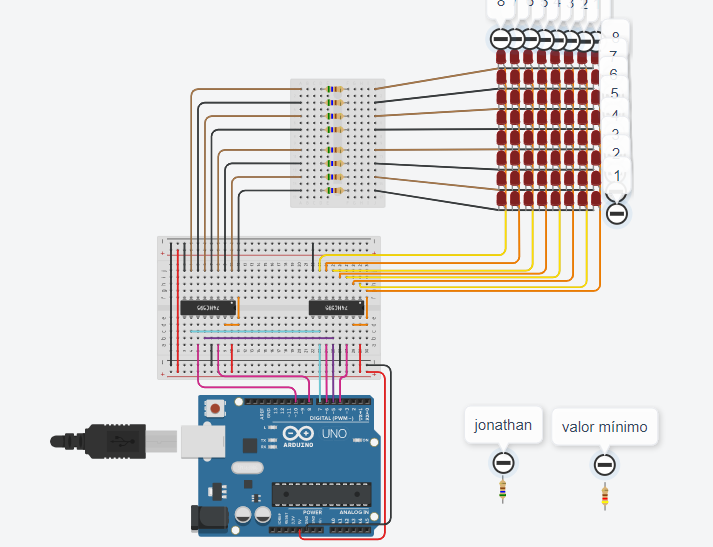
\includegraphics[scale=0.5]{montaje2.png}
\centering
\caption{Montaje mejorado del circuito.}
\label{fig:montaje2}
\end{figure}
 
Martes 20: se crea un menú, y se modifican las funciones verificacion(), e imagen(),  de modo que su integración sea exitosa. Además, se modifican ambas funciones para recibir por parte del usuario el tiempo que desea que estén encendidos los leds, objetivo que se cumplió con la función verificacion(), pero de momento no con imagen(). Además se descubre que al igual como ocurrió con el pin output register clock, es posible integrar en un mismo pin el input (SER) de ambos integrados, y considerando que ya se desarrolló desde el inicio una función para apagar la matriz, se decide en definitiva eliminar el uso del pin digital encargado del clear de los integrados, dándonos como resultado, una matriz de leds controlada con  dos integrados y únicamente 4 pines digitales.

 \begin{figure}[h]
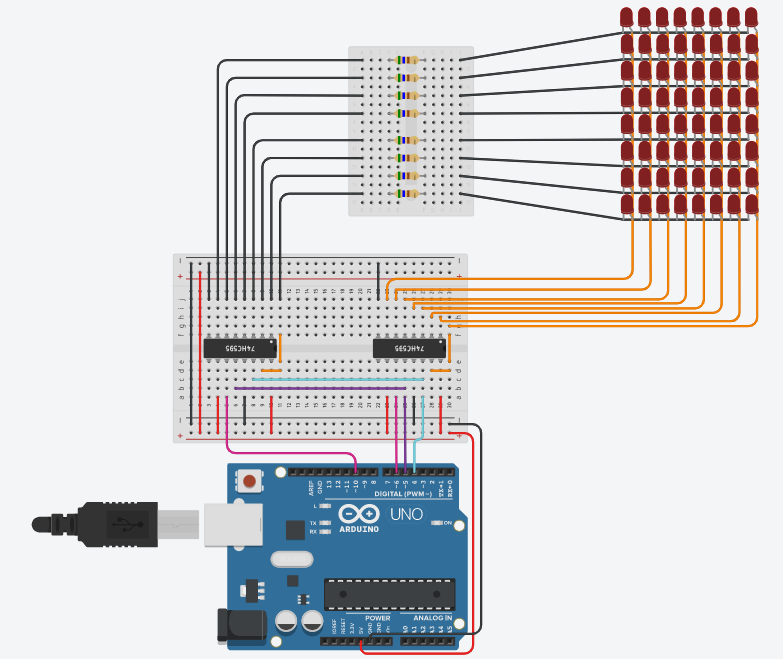
\includegraphics[scale=0.4]{montaje 4 final.png}
\centering
\caption{Montaje usando 4 pines digitales.}
\label{fig:montaje4}
\end{figure}

\newpage
Jueves 22: Se descarta en definitiva el uso de una librería donde se tenga una función para cada letra determinada, se finaliza la función publik, y se pulen detalles de la interfaz con la que interactuará el usuario. Queda pendiente la grabación del video.

\section{Manual de usuario.}
A continuación se presenta el manual de usuario del programa:
\begin{enumerate}
\item Para inicializar el programa damos click en 'código', opcion encerrada en rojo y marcada como "Paso 1" (\ref{fig:paso1}), luego en 'Iniciar simulación' encerrada en verde y marcada como "Paso 2"  (\ref{fig:paso1}), por último damos click en 'monitor en serie' opcion encerrada en azul y marcada como "Paso 3" (\ref{fig:paso1}).
 
 \begin{figure}[h]
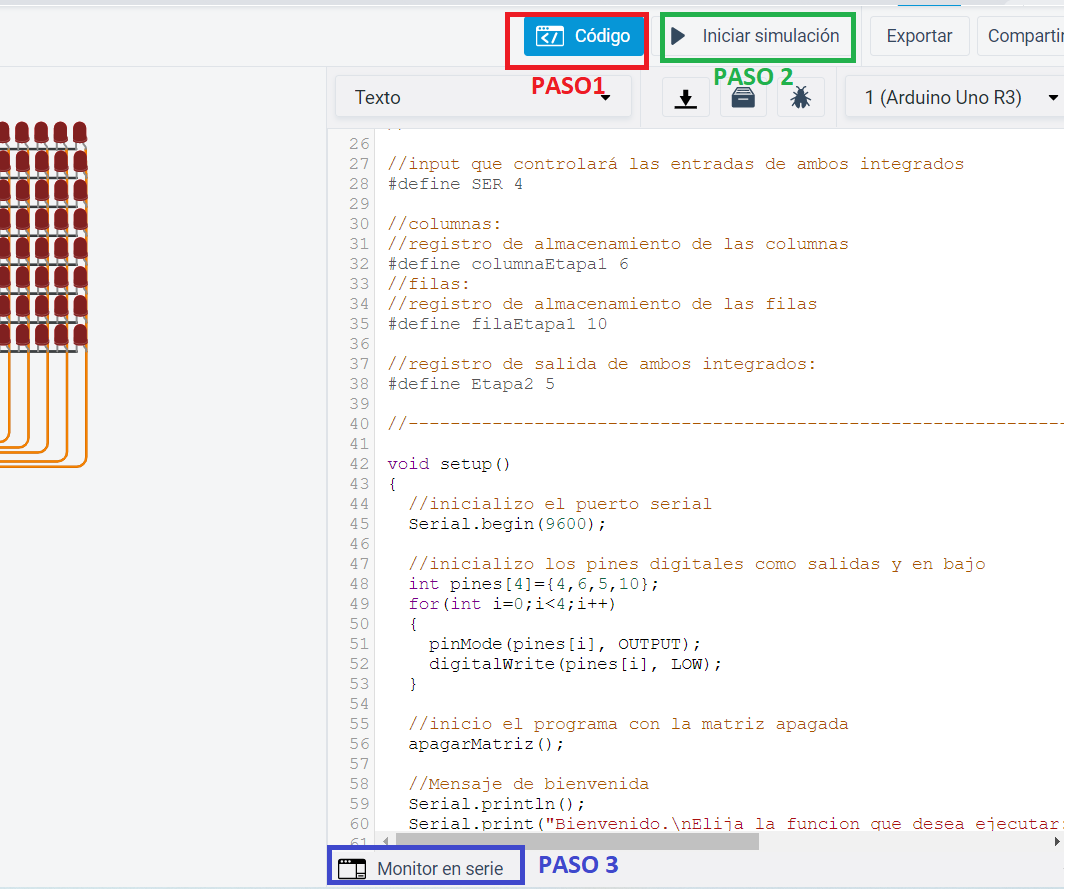
\includegraphics[scale=0.5]{PASO1.png}
\centering
\caption{Iniciar el programa.}
\label{fig:paso1}
\end{figure}

\item Después de iniciar el programa se podrán ver las diferentes opciones que ofrece, el usuario ingresará la opcion que desee mediante el monitor en serie dando click en el espacio marcado con una flecha roja, porteriormente digitando la opción y dando al enter. (\ref{fig:monitorserial}).

\begin{figure}[h]
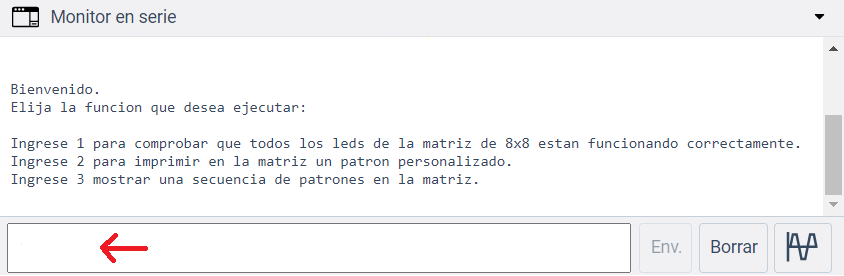
\includegraphics[scale=0.6]{monitorenserie.png}
\centering
\caption{El monitor serial es por donde el usuario ingresa los datos.}
\label{fig:monitorserial}
\end{figure}

\item Al pedirle al programa que ejecute la primera opción, siendo esta la de verificación, nos pide los segundos que se desea ver los LEDs encendidos, este tiempo (en segundos) será el que el usuario desee y se mandará por medio del monitor en serie. La matriz de LEDs quedará encendida en su totalidad por el tiempo que el usuario ingresó anteriormente.

\begin{figure}[h]
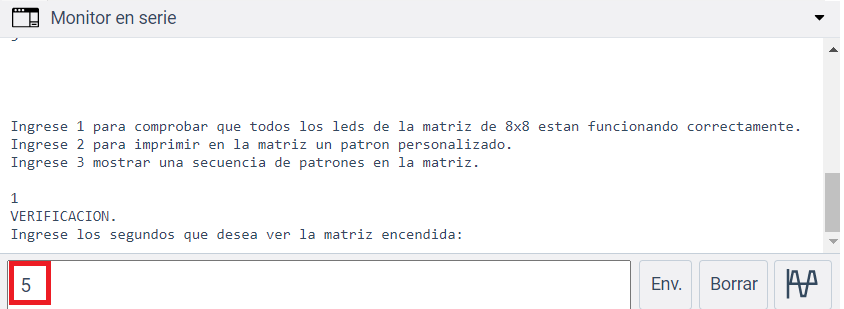
\includegraphics[scale=0.6]{verif.png}
\centering
\caption{Tiempo que ingresa el usuario.}
\label{fig:verif}
\end{figure}

\item En la opción 2, marcada con amarillo (\ref{fig:opcion2}), el usuario podrá ingresar un patrón personalizado, también podrá escoger el tiempo (en segundos) de visualización del patrón estos marcados en naranja en la imagen de ejemplo (\ref{fig:opcion2}), porteriormente se le pedirá al usuario ingresar fila por fila (cada fila se compone de ocho números) el patrón que desea observar (\ref{fig:matrizleds}), estas filas se compondrán de unos y ceros, significando un uno que el led en esa posición se encienda, y un cero que el led en esa posición se apague. El programa le pedirá fila por fila hasta que complete las ocho requeridas.(\ref{fig:matrizleds}),

\begin{figure}[h]
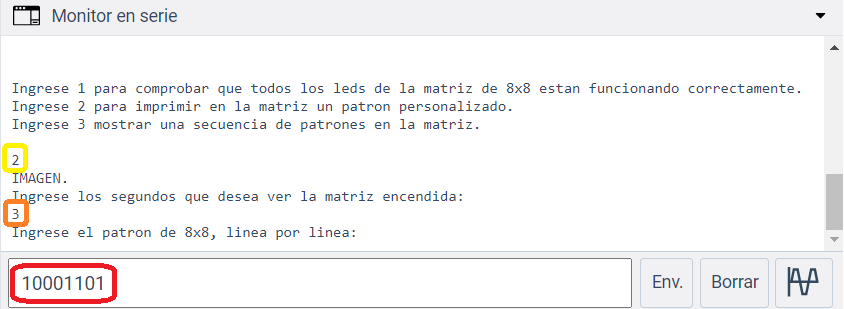
\includegraphics[scale=0.6]{opc2.png}
\centering
\caption{Segunda opcion.}
\label{fig:opcion2}
\end{figure}

\begin{figure}[h]
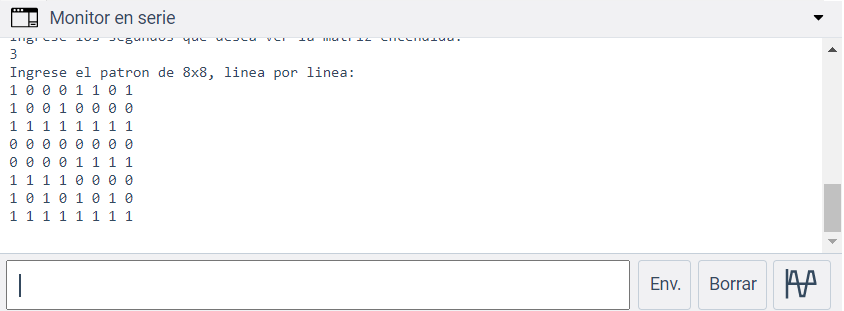
\includegraphics[scale=0.6]{matrizleds.png}
\centering
\caption{Ingresar fila por fila el encendido o apagado de LEDs.}
\label{fig:matrizleds}
\end{figure}

\newpage
\begin{figure}[h]
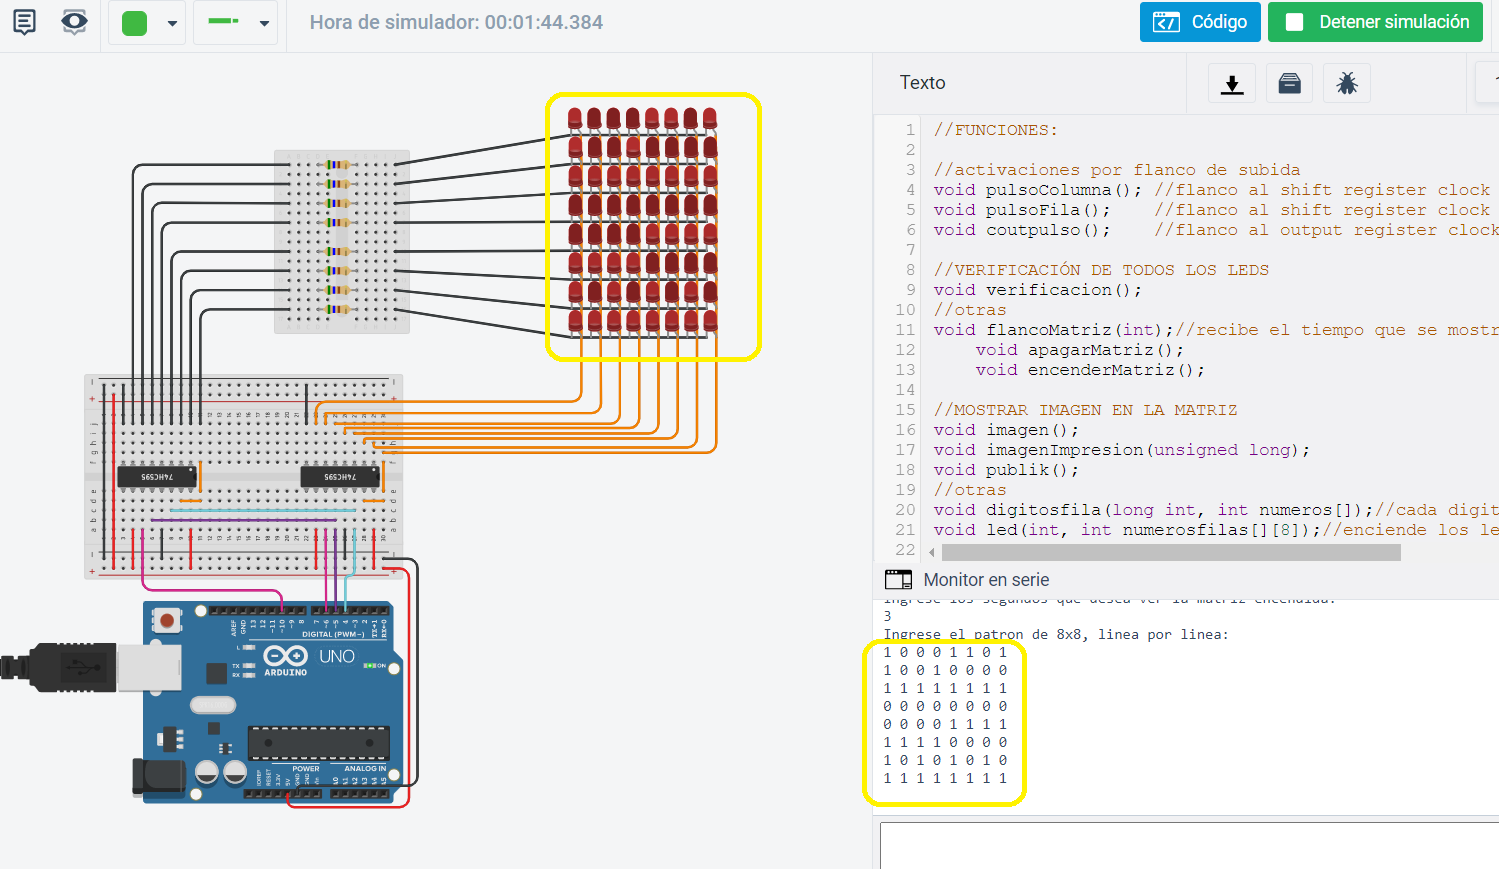
\includegraphics[scale=0.5]{patronper.png}
\centering
\caption{Patrón que se ve en los LEDs después de ingresar fila por fila los unos y ceros que se observan en la figura 12.}
\label{fig:patronper}
\end{figure}

\end{enumerate}


\section{Inclusión de imágenes} \label{imagenes}

En la Figura (\ref{fig:montaje1}), se presenta el primer montaje del circuito. 

Las secciones (\ref{intro}), (\ref{contenido}) y (\ref{imagenes}) dependen del estilo del documento.

\bibliographystyle{IEEEtran}
\bibliography{references}

\end{document}
